\documentclass[tikz,border=12pt]{standalone}
\usepackage[T1]{fontenc}
\usepackage{mathpazo}
\usepackage{amsmath,amssymb}
\usetikzlibrary{arrows.meta, positioning, calc}

\definecolor{stblue}{HTML}{7B97AD}
\definecolor{rwgold}{HTML}{B8995E}
\definecolor{sage}{HTML}{7A9A7E}
\definecolor{dkbrown}{HTML}{3D3530}
\definecolor{wmgray}{HTML}{7B7067}
\definecolor{cream}{HTML}{F9F6F0}
\definecolor{border}{HTML}{D4C9B8}
\definecolor{terracotta}{HTML}{C47A6A}
\definecolor{lavender}{HTML}{907EA0}

\begin{document}
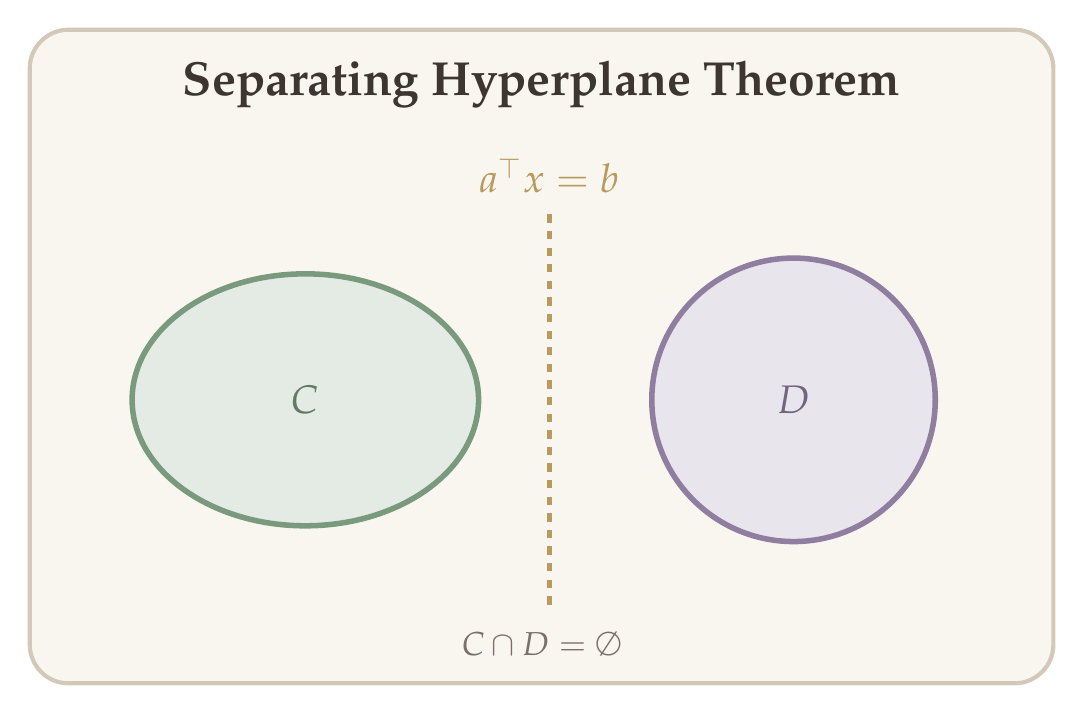
\begin{tikzpicture}[>={Stealth[length=4mm, width=3mm]}]

% Background
\fill[cream, rounded corners=14pt] (-0.5,-0.8) rectangle (12.5,7.5);
\draw[border, line width=1.5pt, rounded corners=14pt] (-0.5,-0.8) rectangle (12.5,7.5);

% Title
\node[text=dkbrown, font=\LARGE\bfseries] at (6,6.8) {Separating Hyperplane Theorem};

% Convex set C (sage, left)
\fill[sage!20] (3,2.8) ellipse (2.2cm and 1.6cm);
\draw[sage, line width=2pt] (3,2.8) ellipse (2.2cm and 1.6cm);
\node[text=sage!80!black, font=\Large\bfseries] at (3,2.8) {$C$};

% Convex set D (lavender, right)
\fill[lavender!20] (9.2,2.8) ellipse (1.8cm and 1.8cm);
\draw[lavender, line width=2pt] (9.2,2.8) ellipse (1.8cm and 1.8cm);
\node[text=lavender!80!black, font=\Large\bfseries] at (9.2,2.8) {$D$};

% Separating hyperplane (dashed vertical line)
\draw[rwgold, line width=2pt, dashed] (6.1,0.2) -- (6.1,5.2);

% Hyperplane label
\node[text=rwgold, font=\Large, anchor=south] at (6.1,5.3) {$a^\top x = b$};

% Annotations
\node[text=wmgray, font=\large] at (6,-0.3) {$C \cap D = \emptyset$};

\end{tikzpicture}
\end{document}
